\textbf{Ejemplo 11}\\
Una persona se comprometió a pagar 250.000 COP en 3 meses, 300.000 COP en 8 meses y 130.000 COP en 15 meses. Ante la dificultad de cumplir con las obligaciones tal como están pactadas solicita una nueva forma de pago así: 60.000 COP hoy, 500.000 COP en 12 meses y el saldo en 18 meses. Suponiendo que la tasa de interés de oportunidad es del 36 \% nominal anual mes vencido, determinar el valor del saldo.
\\
%%%%%%%%%%%%%%%%%%% EJERCICIO 11 %%%%%%

\textbf{Solución.}\\
%La tabla irá centrada
\begin{center}
  \renewcommand{\arraystretch}{1.5}% Margenes de las celdas
  %Creación de la cuadrícula de 3 columnas
  \begin{longtable}[H]{|C{0.3\linewidth}|C{0.3\linewidth}|C{0.30\linewidth}|}
    %Creamos una línea horizontal
    \hline
    %Definimos el color de la primera fila
    \rowcolor[HTML]{FFB183}
    %Título para la primera sección
    \multicolumn{3}{|c|}{\cellcolor[HTML]{FFB183}\textbf{1. Asignación período focal}} \\ \hline
    %Definimos los valores para esta sección
    \multicolumn{3}{|c|}{$pf : 8pmv$} \\ \hline
    %Título para la segunda sección
    \multicolumn{3}{|c|}{\cellcolor[HTML]{FFB183}\textbf{2. Declaración de variables}} \\ \hline
    %Títulos para las subsecciones
    \multicolumn{3}{|c|}{\cellcolor[HTML]{FFB183}\textbf{2.1 Deuda inicial}} \\ \hline
    \multicolumn{1}{|c|}{\cellcolor[HTML]{FFB183}\textbf{Valores monetarios}} &
    \multicolumn{1}{c|}{\cellcolor[HTML]{FFB183}\textbf{Valores no monetarios}} &
    \multicolumn{1}{c|}{\cellcolor[HTML]{FFB183}\textbf{Incógnitas}} \\ \hline
    %Valores de las variables
    $P_1 = 250{.}000$ COP & $n_1 = 3 \textit{ pmv}$ & \\
    $P_2 = 300{.}000$ COP & $n_2 = 8 \textit{ pmv}$ & \\
    $F_3 = 130{.}000$ COP & $n_3 = 15 \textit{ pmv}$ & \\
    
    %Sección 2.2
    \multicolumn{3}{|c|}{\cellcolor[HTML]{FFB183}\textbf{2.2 Deuda equivalente}} \\ \hline
    \multicolumn{1}{|c|}{\cellcolor[HTML]{FFB183}\textbf{Valores monetarios}} &
    \multicolumn{1}{c|}{\cellcolor[HTML]{FFB183}\textbf{Valores no monetarios}} &
    \multicolumn{1}{c|}{\cellcolor[HTML]{FFB183}\textbf{Incógnitas}} \\ \hline
    $P_4 = 60.000$ COP & $n_4 = 0$ pmv &  $F_6 = ? \textit{ COP}$\\
    $F_5 = 500.000$ COP & $n_5 = 12$ pmv &  \\ 
    & $n_6 = 18$ pmv &  \\ 
    & $j = 36\% \textit{ namv}$ & \\
    & $m = 12 \textit{ pmv}$ & \\
    & $i = \frac{36\% \textit{ namv}}{12 \textit{ pmv}}$ & \\ \hline
    %Sección 3
    \rowcolor[HTML]{FFB183}
    \multicolumn{3}{|c|}{\cellcolor[HTML]{FFB183}\textbf{3. Diagrama de flujo de caja}} \\ \hline
    %Inserción de la imagen
    \multicolumn{3}{|c|}{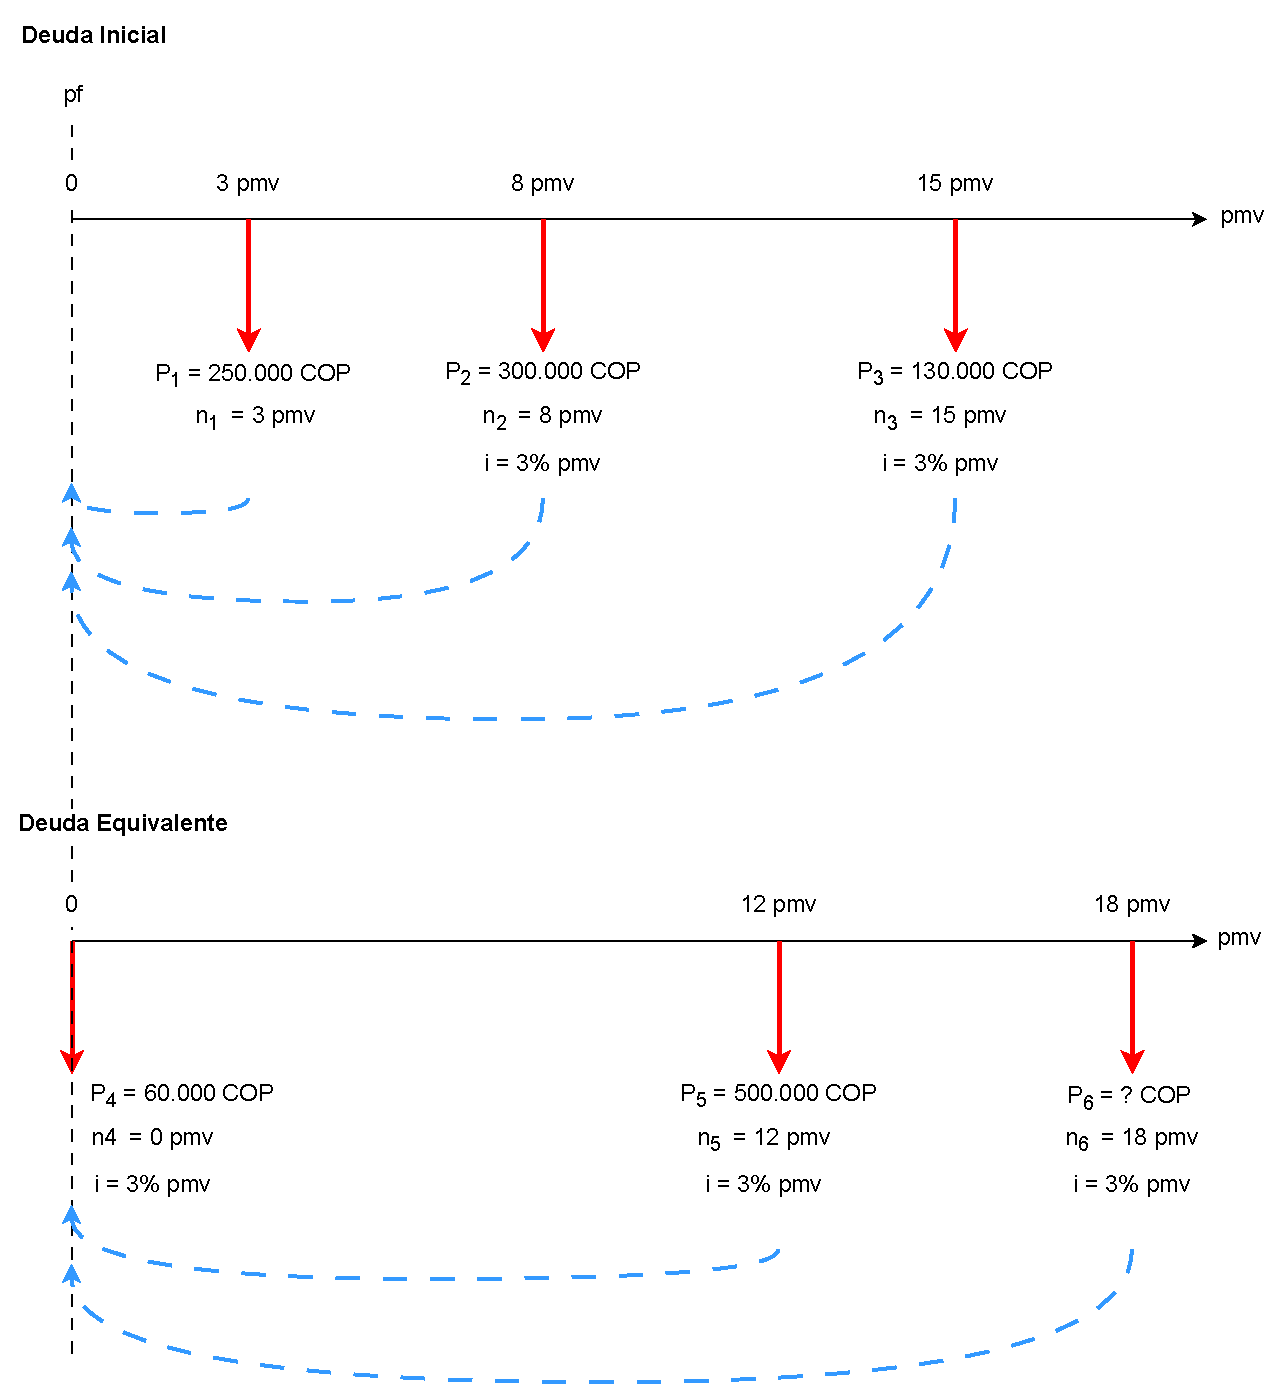
\includegraphics[trim=-5 -5 -5 -5 , scale=0.6]{2_Capitulo/ejemplos/11/Capitulo2_Ejercicio11}} \\ \hline
    %Sección 4
    \rowcolor[HTML]{FFB183}
    \multicolumn{3}{|c|}{\cellcolor[HTML]{FFB183}\textbf{4. Declaración de fórmulas}} \\ \hline
    %Fórmulas
    \multicolumn{3}{|c|}{$F_1 + F_2 + F_3 = F_4 + F_5 + F_6\hspace{0.3cm} \textit{Ecuación de equivalencia}$} \\
    \multicolumn{3}{|c|}{$F = P(1+i)^n\hspace{0.3cm} \textit{Valor futuro}$} \\ \hline
    %Sección 5
    \rowcolor[HTML]{FFB183}
    \multicolumn{3}{|c|}{\cellcolor[HTML]{FFB183}\textbf{5. Desarrollo matemático}} \\ \hline
    %Desarrollo matemático
    \multicolumn{3}{|c|}{$250{.}000 \textit{ COP} (1+0.03)^{3}+ 300{.}000 \textit{ COP} (1+0.03)^8+ 130{.}000 \textit{ COP} (1+0.03)^{15}$} \\
    \multicolumn{3}{|c|}{$= 60{.}000 \textit{ COP} + 500{.}000 \textit{ COP} (1+0.03)^{12}+ F_6 \textit{ COP} (1+0.03)^{18}$} \\ 
    \multicolumn{3}{|c|}{$855{.}748.54 \textit{ COP} = 772{.}880 \textit{ COP} + F_6 \textit{ COP} (1+0.03)^{18}$} \\ 
    \multicolumn{3}{|c|}{$855{.}748.54 \textit{ COP} - 772{.}880 \textit{ COP} = F_6 \textit{ COP} (1.7024)$} \\
    \multicolumn{3}{|c|}{$855{.}748.54 \textit{ COP} - 772{.}880 \textit{ COP} = F_6 \textit{ COP} (1.7024)$} \\
    \multicolumn{3}{|c|}{$\frac{82{.}868.54 \textit{ COP}}{(1.7024)} = F_6 \textit{ COP}$} \\
    \multicolumn{3}{|c|}{$F_{6} = 235{.}549.16 \textit{ COP}$} \\ \hline
    %Sección 6
    \rowcolor[HTML]{FFB183}
    \multicolumn{3}{|c|}{\cellcolor[HTML]{FFB183}\textbf{6. Respuesta}} \\ \hline
    %Respuesta
    \multicolumn{3}{|c|}{$F_{6}=235{.}549.16 \textit{ COP}$} \\ \hline
  \end{longtable}
\end{center}

%%%%%%%%%%%%%%%%%%%%%%%%%%FIN EJERCICIO 1 %%%%%%%%%%%%%%%%%%%%%%%%%%%
